\documentclass[12pt, a4paper]{article}
\usepackage{geometry}
\usepackage{array}
\usepackage{multicol}
\usepackage{multirow}
\usepackage{graphicx}
\usepackage{caption}

\geometry{a4paper, margin=1cm}
\graphicspath{{img}}
\pagenumbering{gobble}
\date{}
\captionsetup[figure]{labelformat=empty}

\title{

  \LARGE{\textbf{LAPORAN}}

  {\vspace{1cm}}

  \large{\textbf{Quiz Perhitungan Subnet IP}}

  {\large{Diajukan untuk Memenuhi Tugas Mata Kuliah Jaringan Komputer}}

  {\vspace{2cm}}

  \normalsize{Radinal Shidiq Saragih (5520123104)}

  \normalsize{Mohammad Hiqmal Ariffansyah (5520123095)}

  \normalsize{Ridho Faatihul Ihsan (5520123106)}

  {\vspace{2cm}}

  {
\includegraphics[scale=2.0]{LogoFakultas.jpeg}}

  {\vspace{3cm}}

  {\large{PROGRAM STUDI TEKNIK INFORMATIKA}}

  {\large{FAKULTAS TEKNIK}}

  {\large{UNIVERSITAS SURYAKANCANA}}

  {\large{CIANJUR}}

  {\small{2024}}
}

\begin{document}
\maketitle

\newpage

\begin{center}
  \section*{PERHITUNGAN IP}
\end{center}

\vspace{1cm}

Diberikan IP address 172.16.0.0/16. Bagilah menjadi 3 subnet yang seimbang dan tentukan:

\begin{enumerate}
    \item Network ID dari setiap subnet
    \item Subnet mask yang digunakan
    \item Broadcast address dari setiap subnet
\end{enumerate}

\textbf{Diketahui:}
\begin{itemize}
    \item IP Address: 172.16.0.0/16
    \item Jumlah subnet: 3
    \item Minimal host per subnet: 500
\end{itemize}

\textbf{Perhitungan:}
\begin{enumerate}
    \item \textbf{Menentukan subnet mask:}
    \begin{itemize}
        \item Karena butuh minimal 500 host, kita perlu 9 bit untuk host (2\^9 = 512 host).
        \item Jika 9 bit untuk host, maka 23 bit untuk network.
        \item Subnet mask: 255.255.254.0 (/23)
    \end{itemize}

    \item \textbf{Menentukan network ID setiap subnet:}
    \begin{itemize}
        \item Subnet 1: 172.16.0.0
        \item Subnet 2: 172.16.2.0 (ditambah 512 alamat dari subnet sebelumnya)
        \item Subnet 3: 172.16.4.0 (ditambah 512 alamat dari subnet sebelumnya)
    \end{itemize}

    \item \textbf{Menghitung broadcast address setiap subnet:} 
    (network ID + ukuran subnet - 1)
    \begin{itemize}
        \item Subnet 1: 172.16.1.255
        \item Subnet 2: 172.16.3.255
        \item Subnet 3: 172.16.5.255
    \end{itemize}
\end{enumerate}

\textbf{Tabel Perhitungan}

\begin{center}
    \begin{tabular}{|c|c|c|c|c|}
        \hline
        \textbf{Subnet} & \textbf{Subnet Mask} & \textbf{Network ID} & \textbf{Broadcast Address} & \textbf{Range IP Host} \\
        \hline
        1 & 255.255.254.0 & 172.16.0.0 & 172.16.1.255 & 172.16.0.1 - 172.16.1.254 \\
        \hline
        2 & 255.255.254.0 & 172.16.2.0 & 172.16.3.255 & 172.16.2.1 - 172.16.3.254 \\
        \hline
        3 & 255.255.254.0 & 172.16.4.0 & 172.16.5.255 & 172.16.4.1 - 172.16.5.254 \\
        \hline
    \end{tabular}
\end{center}

\newpage

\begin{center}
  \section*{TOPOLOGI}
\end{center}

\vspace{1cm}

  Dari hasil perhitungan diatas maka telah topologi sebagai berikut, disini
  digunakan hanya dua vpcs untuk tiap switch namun jumlah maksimal host id yang
  dapat digunakan tetap sama seperti yang telah diperhitungkan sebelumnya.

  \begin{figure}[h]
      \centering
      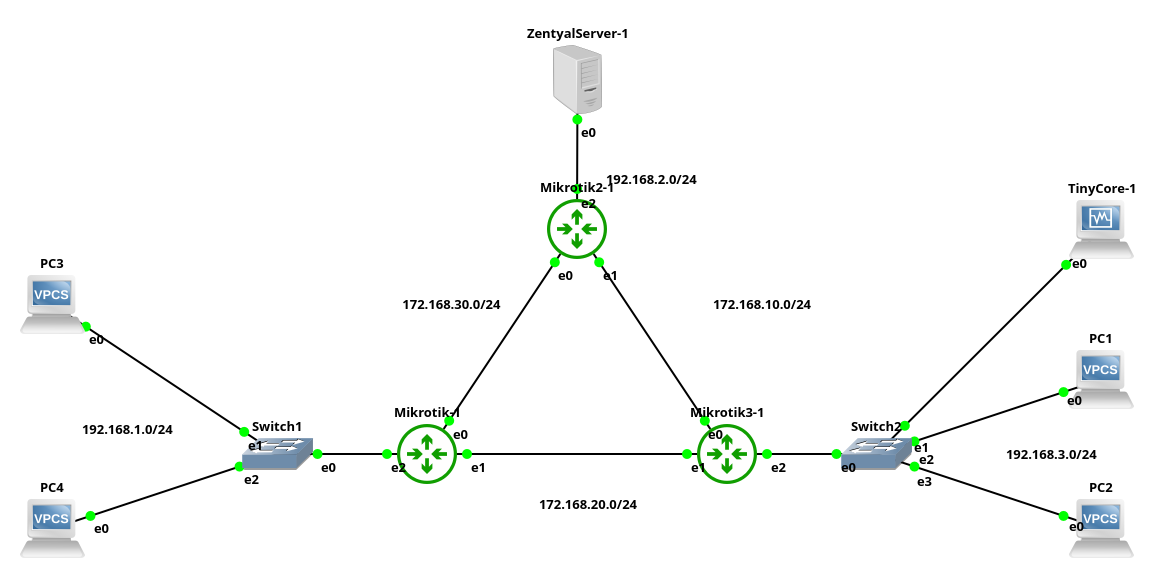
\includegraphics[scale=0.8]{TOPOLOGI.png}
      \caption{Bentuk Topologi}
  \end{figure}

  \begin{enumerate}
    \item Router

      Disini router yang digunakan memiliki 3 port ethernet yang digunakan,
      dan digunakan sebagai konsentrator dari keenam vpcs yang digunakan di
      topologi ini.

      \begin{center}
        \includegraphics[scale=0.6]{ROUTER\_CONF.png}
      \end{center}

    \newpage
    \item Konfigurasi VPCS

      \begin{enumerate}
        \item Subnet 172.16.0.0/23 dan 172.16.1.0/23

          \begin{multicols}{2}
              \includegraphics[scale=0.8]{PC1\_CONF.png}
              \columnbreak
              \includegraphics[scale=0.8]{PC2\_CONF.png}
          \end{multicols}

        \item Subnet 172.16.2.0/23 dan 172.16.3.0/23

          \begin{multicols}{2}
              \includegraphics[scale=0.8]{PC4\_CONF.png}
              \columnbreak
              \includegraphics[scale=0.8]{PC5\_CONF.png}
          \end{multicols}

        \item Subnet 172.16.4.0/23 dan 172.16.5.0/23

          \begin{multicols}{2}
              \includegraphics[scale=0.8]{PC7\_CONF.png}
              \columnbreak
              \includegraphics[scale=0.8]{PC8\_CONF.png}
          \end{multicols}

      \end{enumerate}

    \newpage

    \begin{center}
      \section*{PENGUJIAN PING}
    \end{center}

      \vspace{1cm}

    Dari keenam akan diuji ping dari tiga vpcs, tiap vpcs akan melakukan
    ping terhadap semua vpcs selain dirinya sendiri. Pengujian ini
    bertujuan untuk memastikan konfigurasi telah dilakukan dengan 
    benar dan vpcs yang digunakan dapat saling berkomunikasi.
    Berikut adalah pengujian konektivitas dari VPCS PC1, PC4, dan PC7.

    \begin{enumerate}
      \item PC1

        \begin{center}
              \includegraphics[scale=0.8]{PC1\_PING.png}
        \end{center}
        \newpage

      \item PC4

        \begin{center}
              \includegraphics[scale=0.8]{PC4\_PING.png}
        \end{center}
        \newpage

      \item PC7

        \begin{center}
              \includegraphics[scale=0.8]{PC7\_PING.png}
        \end{center}
        \newpage

    \end{enumerate}

  \end{enumerate}


\end{document}
